\documentclass[a4paper]{article}
\usepackage[T1]{fontenc}
\usepackage{hyperref}
\usepackage[margin=1.5in]{geometry}
\usepackage{graphicx}
\renewcommand{\figurename}{Kadr}

\title{Określanie ilości osób na stoku narciarskim na podstawie nagrań wideo, w celu określenia obciążenia trasy}
\date{}
\author{Michał Rogala, Szymon Stasiak, Przemysław Woźniakowski}

\begin{document}
  \maketitle

\section{Wstęp}
Projekt zrealizowany zostanie w formie aplikacji desktopowej stworzonej z wykorzystaniem technologii .NET Framework. Warstwa graficzna zaimplementowana z użyciem WPF bądź WinForms.
Przedstawiona aplikacja będzie wczytywać pliki do analizy i przetworzenia oraz zapewniać podstawowe możliwości regulacji niektórych parametrów wywołań w celu lepszego dostosowania otrzymanego wyniku do potrzeb użytkownika.

\subsection{Cel}
Określanie ilości osób na stoku narciarskim na podstawie nagrań wideo, w celu określenia obciążenia trasy.

\subsection{Założenia}
W związku z panującą na świecie epidemią, dostęp do transmisji ze stoków jest jednak ograniczony, dlatego też posługiwać będziemy się archiwalnymi nagraniami z serwisu YouTube. Podstawowym materiałem do testów będzie nagranie ze stoku Snoqualmie w USA dostępne w serwisie YouTube pod adresem (\url{https://youtube.com/watch?v=GNV9a4Ilsq8}).\\ Szczególnie wartościowe będą ujęcia zaczynające się około 42. minuty tego nagrania (przykładowe klatki poniżej), zakładamy więc:
\begin{itemize}
\item statyczną kamerę
\item mniej więcej stałą wielkość (procentową względem całości kadru) narciarza
\item dobre warunki atmosferyczne (dobra widoczność, jasność, kontrast)
\item brak dodatkowych elementów ruchomych (wyciągów itp.)
\item małe obciążenie stoku (poniżej 40 osób w dowolnym momencie)
\end{itemize}
Żadne z wymienionych założeń nie musi oznaczać ograniczenia (w szczególności program powinien działać sprawnie dla większej liczby narciarzy), jednak pozwalają określić minimalne wymagania, dla których projekt można uznać za zakończony powodzeniem.\\
W pierwszej części realizacji projektu skupimy się na kadrach widocznych w minutach 44:06 - 46:54 (zdjęcie 1), później jako dodatkowe materiały przeanalizujemy zachowanie dla innych ujęć (przykładowe zdjęcia 2 i 3).
\begin{figure}
  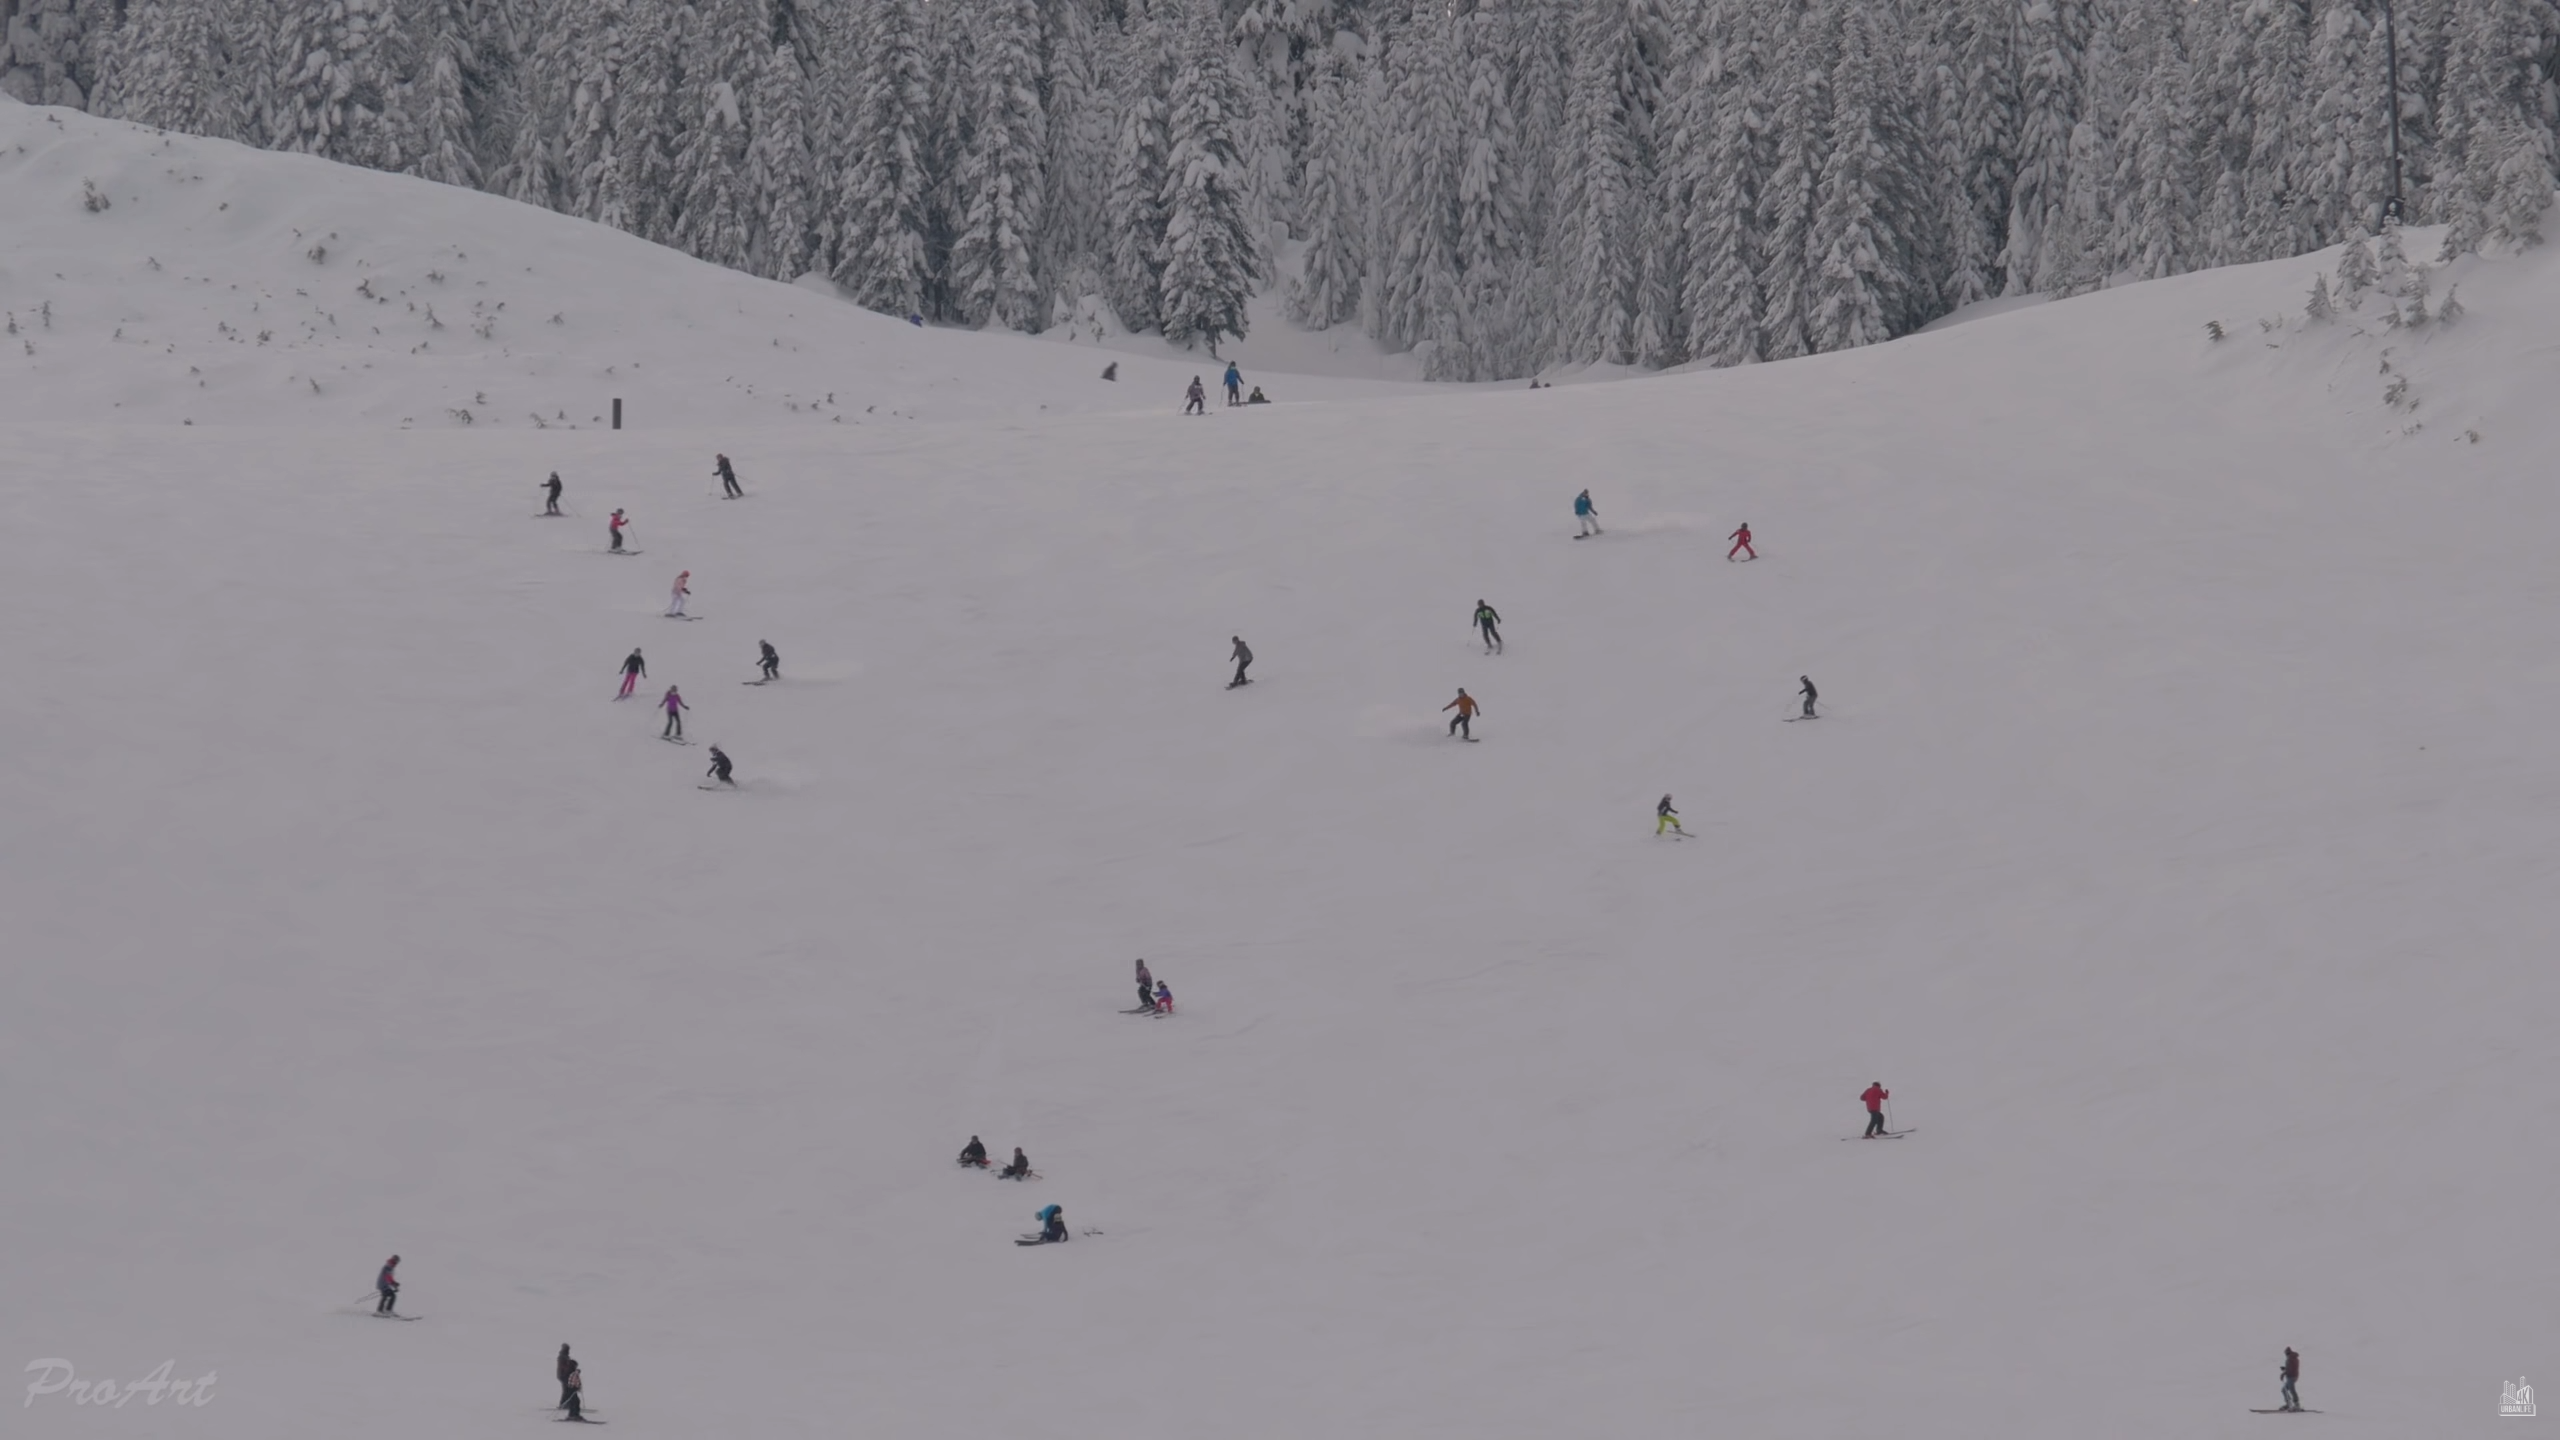
\includegraphics[width=\linewidth]{resources/img1.png}
  \caption{Podstawowe ujęcie}
\end{figure}
\begin{figure}
  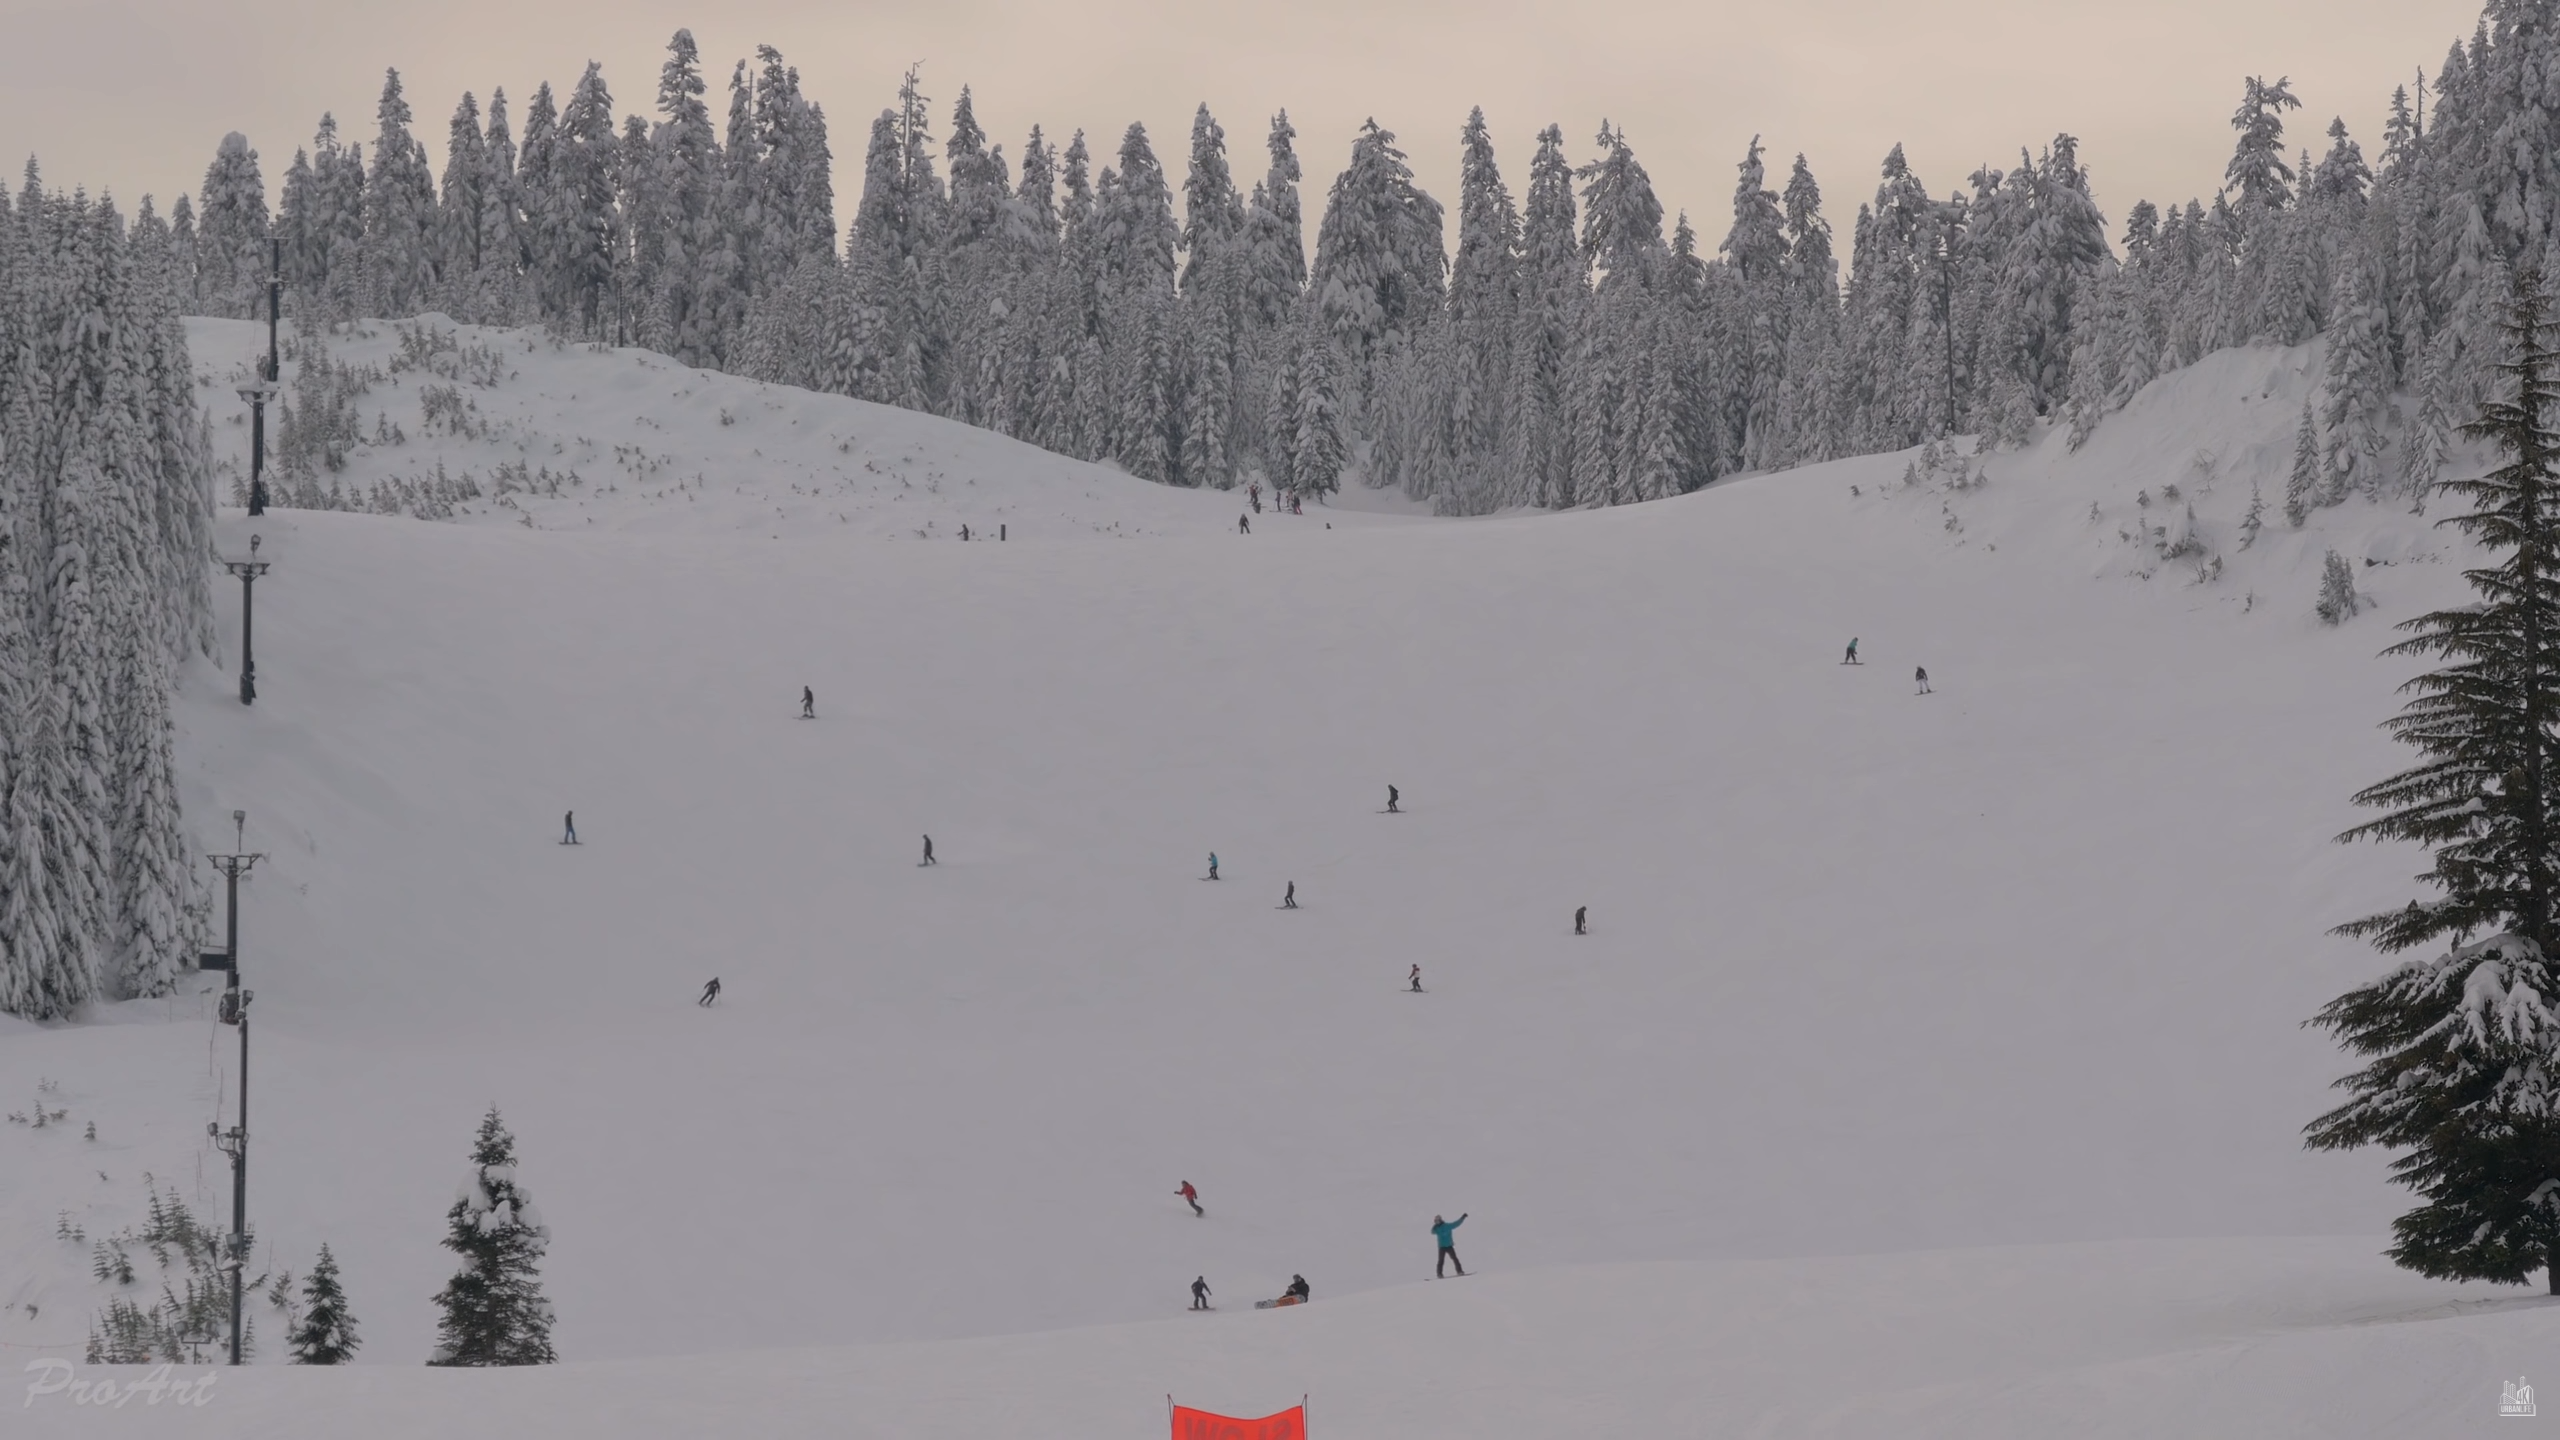
\includegraphics[width=\linewidth]{resources/img2.png}
  \caption{Ujęcie z dalszej perspektywy}
\end{figure}
\begin{figure}
  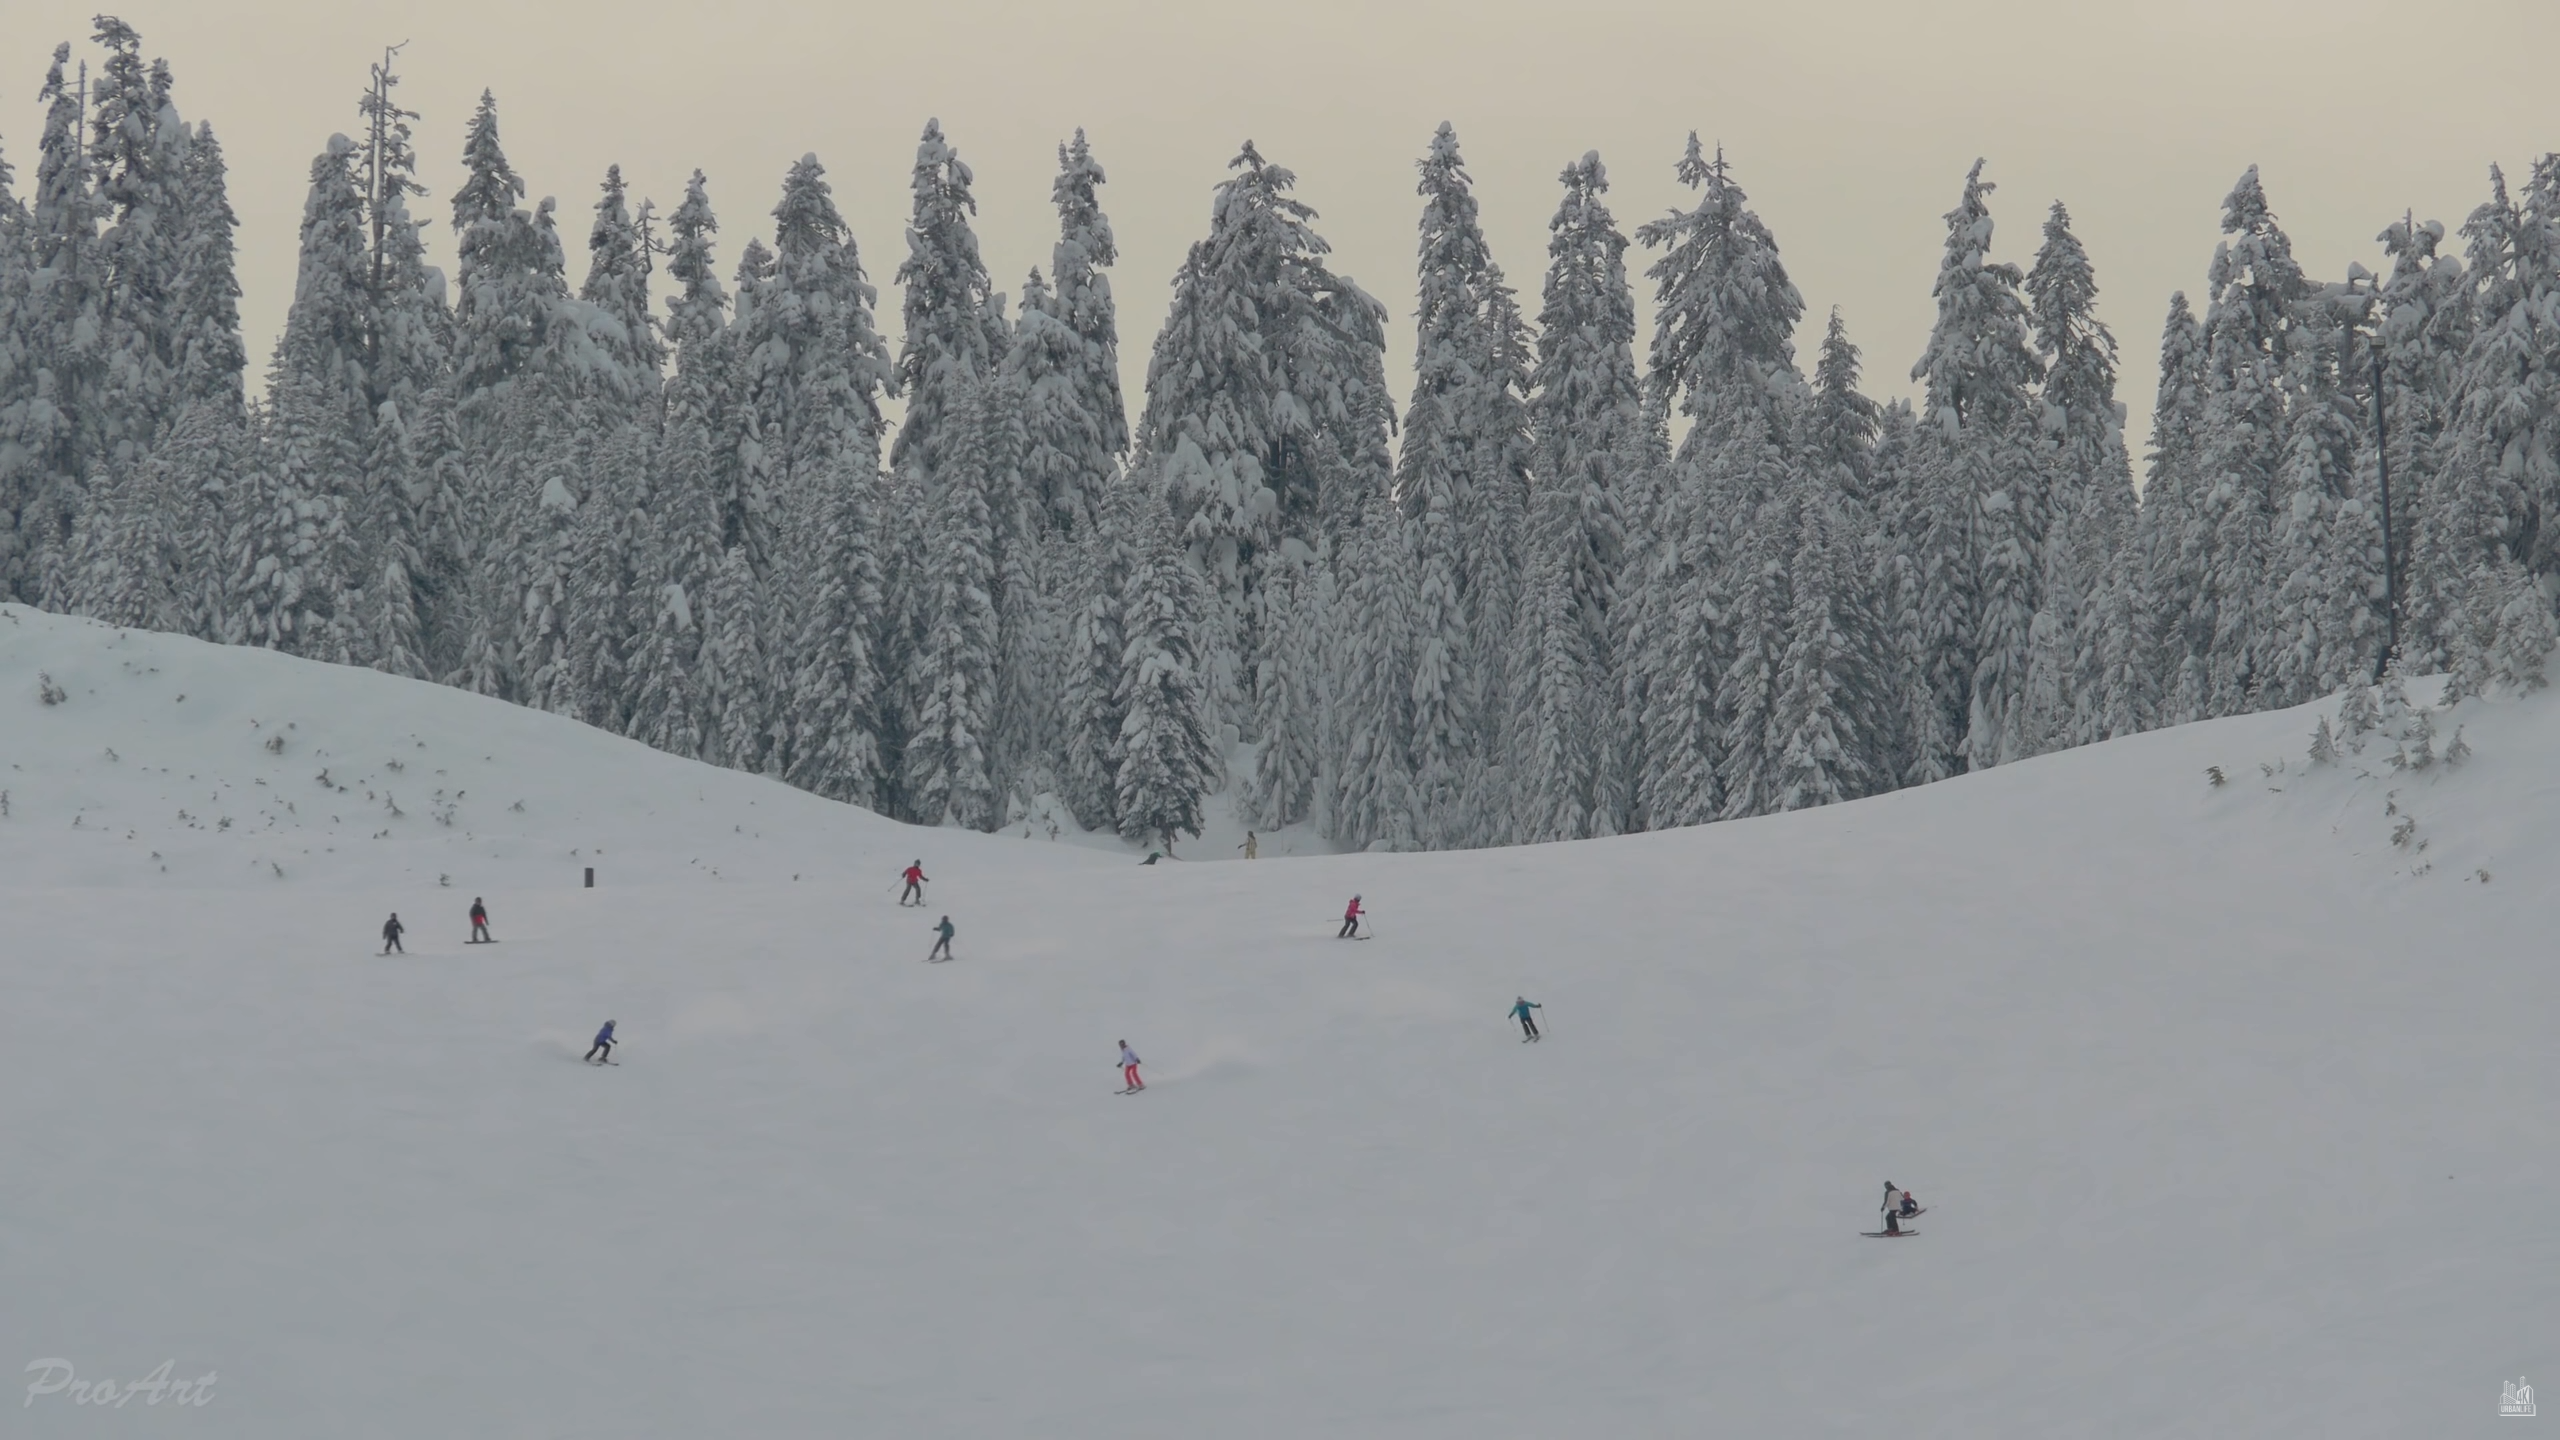
\includegraphics[width=\linewidth]{resources/img3.png}
  \caption{Większa powierzchnia tła}
\end{figure}

\subsection{Metody}
\begin{enumerate}
\item \textbf{Detekcja i śledzenie ruchu używając obrazu tła i różnic między kolejnymi klatkami materiału wideo} (Motion Detection and Tracking using Background Subtraction and Consecutive Frames Difference Method)
	\begin{enumerate}
	\item Obraz tła (pusty stok) wgrany z pliku
	\item Obraz tła uzyskany jako średnia z wielu klatek nagrania
	\end{enumerate}
\item \textbf{Metoda naiwna} (Blob detection) – wykrywanie ciemnych plan na kolejnych klatkach
	\begin{enumerate}
	\item Zróżnicowanie wyników w zależności od parametrów – zakresy wielkości „plam” uznawanych za narciarza, progi kolorów
	\end{enumerate}
\end{enumerate}	

\subsection{Spodziewane efekty}
Wszystkie z powyższych metod powinny radzić sobie na stokach z małym zagęszczeniem ruchu (takimi jak stok wymieniony we wstępie), jednak narciarze znajdujący się blisko siebie mogą stanowić problemy.\\
Najlepsze efekty powinna dawać metoda \textit{1a}. Metoda naiwna przy nieodpowiednim określeniu parametrów może być bardziej podatna na elementy tła a także jasne kolory narciarzy oraz ciemne plamy na śniegu.\\
Wstępnie zakładamy, kilka-kilkanaście klatek przerobionych na sekundę. Celem jest uzyskanie efektu tempa zbliżonego do rzeczywistego nagrania, a więc optymalna ilość przetwarzanych klatek będzie dobrana zależna od czasu przetwarzania jednej klatki. Część klatek będzie pomijana w analizie w celu przyśpieszenia działania.

\subsection{Plan}
\begin{enumerate}
\item Dogłębna analiza metod, dostępnych opracowań i podział zadań
\item Przygotowanie odpowiednich nagrań wideo i ich preprocessing (jeśli potrzebny), wyizolowanie ujęć pustego stoku do metody \textit{1a}
\item Podstawowa implementacja metod i tworzenie warstwy graficznej, wstępne wyniki
\item Ulepszanie, optymalizacja
\item Testy na różnych nagraniach, porównanie metod
\item Raport końcowy
\end{enumerate}


\end{document}

